% !TEX program = xelatex
% 竞赛版 —— 覆盖第一阶段（任务1–3 + 三项拓展）与第二阶段（评审意见三项优化）
% 编译：xelatex main.tex （连续两次）
\documentclass[11pt,a4paper]{ctexart}

\usepackage[a4paper,left=2.4cm,right=2.4cm,top=2.6cm,bottom=2.6cm]{geometry}
\usepackage{amsmath,amssymb,bm}
\usepackage{graphicx}
\usepackage{booktabs}
\usepackage{multirow}
\usepackage{makecell}
\usepackage{array}
\usepackage{caption}
\usepackage{enumitem}
\usepackage{xcolor}
\usepackage[hidelinks]{hyperref}
\usepackage{cleveref}
\usepackage{indentfirst}
% 圈码 ①-⑥ 与 ⇒ 的缺字形修复（2026-09-25 外部体检查出：成品 PDF 里 46 处静默消失）
% 单靠 \xeCJKDeclareCharClass 不够——中文字体有 ①-⑥ 但没有 ⇒，故另配 newunicodechar
\usepackage{newunicodechar}
\xeCJKDeclareCharClass{CJK}{"2460 -> "24FF}
\newunicodechar{⇒}{\ensuremath{\Rightarrow}}

\graphicspath{{../figures/}}
\captionsetup{font=small,labelfont=bf}
\setlength{\parindent}{2em}
\linespread{1.15}
\emergencystretch=2em
% cleveref 中文名（否则输出英文小写 "fig. 1" / "table 1"）
\crefname{figure}{图}{图}\Crefname{figure}{图}{图}
\crefname{table}{表}{表}\Crefname{table}{表}{表}
\crefname{equation}{式}{式}\Crefname{equation}{式}{式}
% 注意：不要给 section 设中文 crefname —— 会触发 "Extra \endcsname"。
% 章节引用一律写成「第 \ref{sec:xxx} 节」。


\title{\bfseries 存算一体芯片中非线性误差对推理精度的影响研究}
\author{黄奕皓\\[2pt] \small 中国科学院大学 计算机科学与技术，北京\\ \small \texttt{huangyihao24@mails.ucas.ac.cn}}
\date{}

\begin{document}
\maketitle

\vspace{-1.2em}
\begin{abstract}
\noindent
存算一体架构把乘累加运算放进模拟存储阵列，代价是模拟器件的非理想特性直接进入计算通路。
本文将输入侧的非线性失真建模为逐样本归一化后的三次多项式 $y=\alpha\hat{x}^3+(1-\alpha)\hat{x}$，
在 CIFAR-10 上对浅层纯前馈（SimpleCNN, 0.24M）、深层纯前馈（VGG-11, 9.2M）
与深层残差（ResNet-18, 11.2M）三类架构，完成了敏感性分析、非线性感知训练与鲁棒性增强三项任务，
以及跨架构、跨扰动类型、多误差源三项拓展研究。

主要结果如下。\textbf{任务1}：正向失真（$\alpha>0$）的破坏力在浅层与中层主干上强于负向
（SimpleCNN 上为 3.4 倍，以 $|\alpha|=0.3$ 的跌幅计），
误差从浅层向深层累积，残差连接是误差放大器——$\alpha=+0.3$ 时 ResNet-18 从 92.09\% 掉到 17.08\%，
跌幅 75.01 个百分点，显著重于 VGG-11（跌至 36.70\%）与 SimpleCNN（跌至 55.08\%）。
\textbf{任务2}：非线性感知训练在纯前馈网络上有效（Scratch 策略 $\alpha=+0.3$ 分别提升 9.15 与 8.04 个百分点），
但在残差网络上失效甚至退化（$-1.44$）；极限失真下的效果与注入点数量负相关（5$\to$9$\to$18 点）。
\textbf{任务3}：在感知训练基础上叠加"残差校准模块 $+$ 分层加权采样"，把 SimpleCNN 的 $\alpha=+0.3$
从 55.08\% 提升到 \textbf{68.76\%}；消融显示分层加权是贡献最大的单项（$+5.13$），
非对称采样的边际贡献仅 $+0.38$。

\textbf{拓展与第二阶段}：跨架构对比显示脆弱性随深度与残差连接递增；
高斯噪声与非线性失真的破坏机制不可通用迁移（ResNet-18 上两者甚至完全反转）；
量化与非线性联合作用呈现三分格局——SimpleCNN 超加性恶化（$\Delta=-7.23$）、
VGG-11 次加性即 Dithering（$\Delta=+7.82$）、ResNet-18 地板效应（$\Delta=+1.05$）。
第二阶段的三项工作进一步给出：非线性感知训练的鲁棒性\textbf{严格限定在训练分布内}，
正向外推在 $\alpha\approx0.4$ 处归零并转为劣势（$\alpha=+0.5$ 时 $-10.77$）而负向保持；
Dithering 的机理是\textbf{离散化分布重塑}（分类器输入峰度从 0.110 恢复到 0.214）
配合 MaxPool 架构载体，\textbf{与随机抖动无关}——这修正了第一阶段给出的"随机共振"解释与注噪建议；
增强方案可完整迁移至深层网络，VGG-11 在 15 个扫描点上全胜三条基线，且干净精度零牺牲。

\vspace{0.6em}
\noindent\textbf{关键词：} 存算一体；非线性失真；非线性感知训练；残差校准；Dithering；量化误差
\end{abstract}

\vspace{0.4em}
\noindent\textbf{范围声明}：本稿覆盖\textbf{第一、二阶段}的工作（CIFAR-10 上的任务 1--3、三项拓展与评审意见三项优化）；
第三阶段起的跨数据集与跨架构工作（CIFAR-100、VGG-11 / ResNet-18 主干）见同期报告，\textbf{不在本稿范围内}。

\section{引言}

\subsection{赛题背景}

传统冯·诺依曼架构下，神经网络推理时数据在存储与计算单元之间反复搬运，
形成功耗与带宽上的"存储墙"。存算一体（Compute-in-Memory, CiM）技术把乘累加运算直接嵌入存储阵列内部，
大幅降低搬运开销~\cite{cim_survey,puma}。但基于 SRAM/Flash 等模拟器件实现的阵列
易受器件失配、跨导放大器增益非线性、工艺偏差与温度漂移的影响，
使乘累加呈现输入相关的非线性特性。

这类误差有一个区别于常见扰动源的性质：它是\textbf{确定性的、与输入幅度相关}的系统误差，
而不是零均值、与信号无关的随机扰动。它逐层累积，并且不能用"多训几轮"来消除。
本文的全部工作围绕一个具体问题展开：\textbf{在这种失真下，模型的精度为什么会退化，
以及什么样的算法手段能真正提升它的容忍能力。}

\subsection{失真模型}

按赛题给定形式，把归一化输入与电路实际响应之间的映射建模为三次多项式：
\begin{equation}
y = \alpha\,\hat{x}^3 + (1-\alpha)\,\hat{x},
\qquad
\hat{x} = \frac{x}{\|x\|_\infty},
\label{eq:distortion}
\end{equation}
其中 $\hat{x}$ 按 batch 维\textbf{逐样本}做无穷范数归一化，避免样本间串扰；
失真通过前向钩子挂在每一个 \texttt{Conv2d} 与 \texttt{Linear} 算子的\textbf{输入侧}，逐层注入。
$\alpha$ 刻画非线性强度，$\alpha=0$ 退化为恒等映射；
$\alpha>0$ 时正输入被放大、负输入被压缩，$\alpha<0$ 时相反。

\subsection{研究框架}

本文的工作分为两个阶段，共六个部分：

\begin{center}
\small
\begin{tabular}{llc}
\toprule
阶段 & 内容 & 对应节号 \\
\midrule
一 & 任务1：非线性误差的敏感性分析 & 第 \ref{sec:task1} 节 \\
一 & 任务2：非线性感知训练（NAT） & 第 \ref{sec:task2} 节 \\
一 & 任务3：鲁棒性增强方法设计 & 第 \ref{sec:task3} 节 \\
一 & 拓展1--3：跨架构 / 跨扰动类型 / 多误差源 & 第 \ref{sec:ext123} 节 \\
\midrule
二 & 优化一：$\alpha$ 扫描范围扩展与外推边界 & 第 \ref{sec:ext4} 节 \\
二 & 优化二：Dithering 效应的定量机理解析 & 第 \ref{sec:ext5} 节 \\
二 & 优化三：增强方案向深层网络的迁移 & 第 \ref{sec:ext6} 节 \\
\bottomrule
\end{tabular}
\end{center}

第二阶段的三项工作对应评审意见的三条子建议，构成"发现问题 $\to$ 解释机理 $\to$ 修复验证"的闭环：
优化一测出现有防御手段的有效边界在哪里；优化二对第一阶段发现的反常现象给出定量判决，
并\textbf{修正第一阶段给出的错误解释}；优化三把最优防御方案迁移到深层网络，
其结果反过来修复了优化一发现的外推短板。

\subsection{实验口径}

除非特别说明，全部实验遵循统一口径：数据集为 CIFAR-10~\cite{cifar}（10 类，全量测试集 10\,000 张）；
评估用 best 权重、纯推理；训练用 SGD（动量 0.9、权重衰减 $10^{-4}$）；
$\alpha$ 的扫描点为 $\{-0.3,-0.2,-0.1,0,+0.1,+0.2,+0.3\}$，
部分外推实验使用 15 点（$\pm0.6$ 至 $0$）。
三个主干为 SimpleCNN（0.24M，4 卷积 + 2 MaxPool）、
VGG-11（9.2M，8 卷积 + 5 MaxPool）~\cite{vgg}
与 ResNet-18（11.2M，含残差连接）~\cite{resnet}。

全部数值均由脚本从实验产物文件现读，并用同一条自检把关：强度扫描文件里 $\alpha=0$ 的行
必须等于同目录训练指标文件记录的最优测试精度（容差 0.01）。
\textbf{适用与例外}：由新训练模型产出的行（任务 1--3、优化三）全部通过该自检，
在全局台账 \texttt{results\_master.csv} 中记为 PASS；\textbf{拓展 2、拓展 3、优化一、优化二不适用}——
它们复用既有权重（没有可配对的指标文件）或是位宽扫描而非强度扫描，
其读数直接取自产物表本身。

\section{任务1：非线性误差的敏感性分析}
\label{sec:task1}

\subsection{破坏力有多大}

\cref{fig:c01} 给出三个干净模型在七个失真强度下的精度。
$\alpha=+0.3$ 时三个模型分别跌 29.82、53.10、75.01 个百分点；
负侧的跌幅在 SimpleCNN 与 VGG-11 上小得多（8.84 与 37.97），
但 \textbf{ResNet-18 两侧几乎同样重}（$\alpha=-0.3$ 时跌 79.71，甚至略重于正侧）。

\begin{figure}[t]
\centering
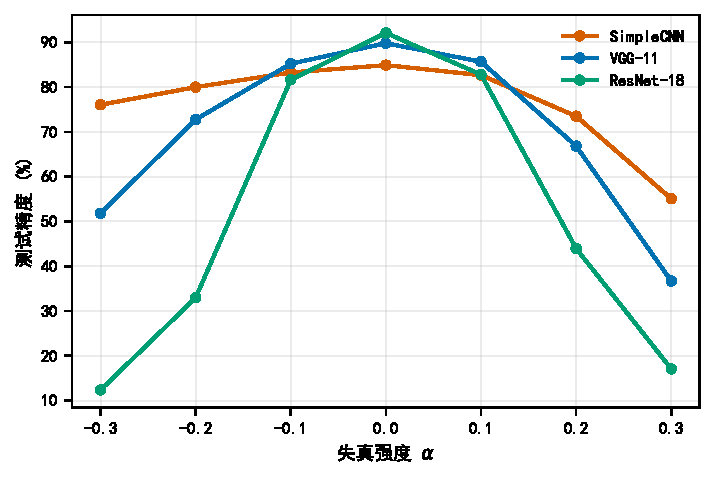
\includegraphics[width=0.72\textwidth]{C01_task1_sensitivity.pdf}
\caption{三个架构的非线性敏感性（CIFAR-10）。
正向失真的破坏力大于负向（SimpleCNN 与 VGG-11 上明显；ResNet-18 上两侧几乎同样重，
见正文），且跌幅随深度与残差连接递增。
全量测试集、best 权重、纯推理。数据：\texttt{outputs/task1\_*/alpha\_sensitivity.csv}。}
\label{fig:c01}
\end{figure}

把正向与负向的破坏力之比按容量排开（以 $|\alpha|=0.3$ 的跌幅计）：
SimpleCNN \textbf{3.4}、VGG-11 \textbf{1.40}、ResNet-18 \textbf{0.94}——
\textbf{方向性随深度衰减，在最深的主干上完全消失}。
SimpleCNN 上的这个比值是后续所有训练策略与采样设计的动机来源。

\subsection{误差往哪里累积}

把"哪个位置受损最重"细分为两类问题后，结论不同：

\begin{itemize}[leftmargin=2em,itemsep=2pt]
  \item \textbf{观测位置}：全层失真时，最深处的 fc 层输出偏移最大
        （与干净输出的余弦相似度仅 \textbf{0.895}），浅层 conv1/conv2 几乎不受影响（余弦 $>0.99$）。
        也就是说误差从浅层向深层\textbf{累积}，fc 是汇聚点。
  \item \textbf{注入位置}：把失真单独施加到某一层时，情况并不相同。
        单层注入的探针显示，最敏感的是中间层卷积，而 fc 单点注入的影响很小。
\end{itemize}

这两者并不矛盾——fc 之所以偏移最大，是因为它承接了前面所有层累积的误差，
而不是因为它自己对失真最敏感。这一区分直接决定了任务3 的设计：
校准模块应当\textbf{作用于误差的累积节点}，而不只是最末端。

\section{任务2：非线性感知训练}
\label{sec:task2}

\subsection{设计}

非线性感知训练（NAT）的思路是在训练阶段就让模型"见过"失真：
每个 batch 从 $\alpha\sim U[-0.3,0.3]$ 均匀采样并注入所有层，
而验证与测试阶段保持干净（$\alpha=0$），从而考察模型的泛化鲁棒性。
本文对比两种策略：在预训练干净权重上\textbf{微调}（Fine-tuning，学习率 $10^{-3}$），
与\textbf{从头训练}（Scratch，学习率 $10^{-2}$），在同一 epoch 预算下比较。

\subsection{结果：NAT 的效果强烈依赖架构}

\begin{figure}[t]
\centering
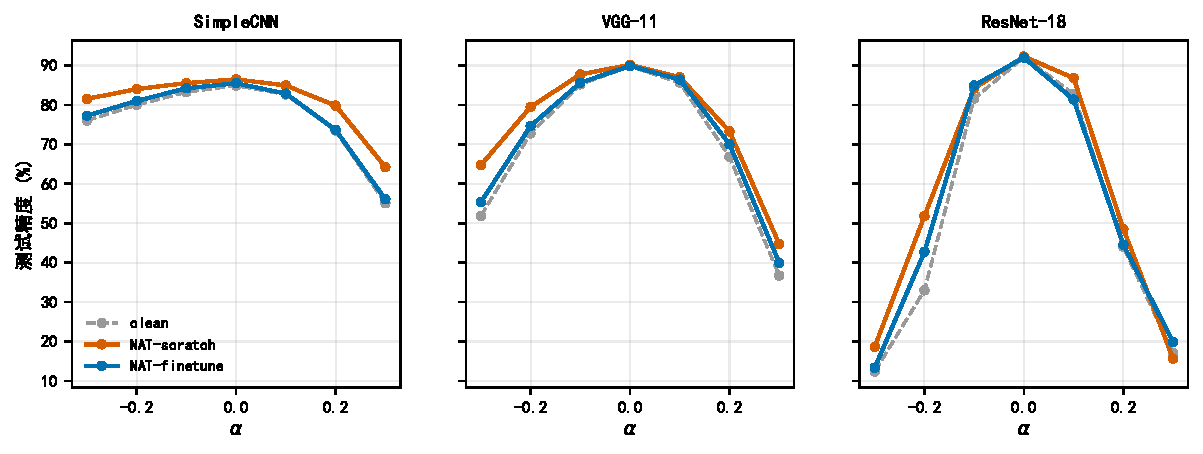
\includegraphics[width=0.98\textwidth]{C02_task2_nat.pdf}
\caption{非线性感知训练在两个策略下的效果（CIFAR-10）。
虚线为干净模型基线，橙色为从头训练（Scratch），黄色为微调（Finetune）。
Scratch 在两种纯前馈架构上全面占优；在残差网络上极限正向失真处出现反转。
数据：\texttt{outputs/task2\_*/\{scratch,finetune\}/alpha\_sensitivity.csv}。}
\label{fig:c02}
\end{figure}

\begin{table}[t]
\centering
\caption{非线性感知训练在 $\alpha=+0.3$ 上的提升（相对同架构干净模型，单位 pp）}
\label{tab:nat}
\small
\begin{tabular}{lccc}
\toprule
架构（注入点数） & 干净精度 & NAT-Scratch & NAT-Finetune \\
\midrule
SimpleCNN（5） & 84.90 & \textbf{+9.15} & +1.00 \\
VGG-11（9） & 89.80 & \textbf{+8.04} & +3.26 \\
ResNet-18（18） & 92.09 & $\mathbf{-1.44}$（退化） & +2.81 \\
\bottomrule
\end{tabular}
\end{table}

\cref{tab:nat} 与 \cref{fig:c02} 给出三条规律：

\textbf{(1) 纯前馈网络上 Scratch 全面占优。}
SimpleCNN 从 55.08\% 提升到 64.23\%，VGG-11 从 36.70\% 提升到 44.74\%。
微调的效果明显较弱（$+1.00$ / $+3.26$），原因是预训练权重携带的"干净特征偏见"
难以在低学习率下被消除。

\textbf{(2) 残差网络上极限正向失真不可救。}
ResNet-18 的 Scratch 策略在 $\alpha=+0.3$ 上反而比干净模型差 1.44 个百分点。
它在失真环境中从零塑造了全部 18 个卷积层，过度适应了极端环境，
反而丧失了从被污染信号中提取残差信息的能力。
相对地，微调因为限制了权重更新幅度、保留了干净特征的编码能力，
在这一点上反常地优于 Scratch（19.89\% vs 15.64\%）。

\textbf{(3) 效果与注入点数量负相关。}
三个架构的注入点数为 5、9、18，$\alpha=+0.3$ 上的 Scratch 提升依次递减
（$+9.15 \to +8.04 \to -1.44$）。
这提示失真信号的累积存在一个临界规模：当它需要穿过 10 个以上的注入点时，
训练端已经无法有效补偿。

值得注意的是，NAT 在\textbf{中等失真}上仍然很有效：ResNet-18 在 $\alpha=-0.2$ 处
从 32.98\% 提升到 51.82\%（$+18.84$），是全部单项实验中最大的提升。
失效只发生在正侧极限。

\section{任务3：鲁棒性增强方法设计}
\label{sec:task3}

\subsection{三种互补的增强方案}

任务1 给出了两个可操作的线索（误差在深层累积、正侧更致命），任务2 给出了一个有效但不够的基线。
在这一基础上叠加三种互补的方法：

\begin{center}
\small
\begin{tabular}{clp{7.2cm}}
\toprule
方案 & 类型 & 核心逻辑 \\
\midrule
A & 架构增强 & 在全局池化之后、分类器之前插入\textbf{残差校准模块}（瓶颈 MLP），
              学习"失真特征 $\to$ 干净特征"的补偿映射；残差连接保证最坏情况退化为恒等映射 \\[2pt]
B & 训练策略 & \textbf{分层加权采样}：浅层用轻失真 $\alpha\in[-0.15,0.15]$，
              深处用强失真固定 $\pm0.3$；精准打击累积瓶颈，同时保护浅层特征 \\[2pt]
C & 采样策略 & \textbf{非对称采样}：按 70\%/30\% 的概率偏向正侧，
              基于任务1 测得的正向破坏力更强这一事实 \\
\bottomrule
\end{tabular}
\end{center}

三个消融配置依次叠加：Exp1（仅 A）、Exp2（A $+$ B）、Exp3（A $+$ B $+$ C）。

\subsection{消融结果}

\begin{figure}[t]
\centering
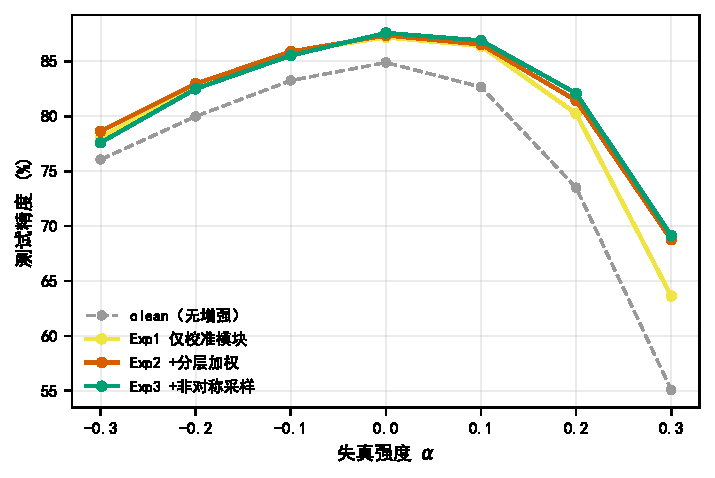
\includegraphics[width=0.72\textwidth]{C03_task3_ablation.pdf}
\caption{鲁棒性增强方案的消融阶梯（CIFAR-10 / SimpleCNN）。
虚线为无增强的干净模型；Exp1 仅含残差校准模块，Exp2 叠加分层加权采样，
Exp3 再叠加非对称采样。数据：\texttt{outputs/task3\_simplecnn/Exp*/alpha\_sensitivity.csv}。}
\label{fig:c03}
\end{figure}

\begin{table}[t]
\centering
\caption{消融阶梯（CIFAR-10 / SimpleCNN，各配置均为 120 epoch 从头训练）}
\label{tab:ablation}
\small
\begin{tabular}{lcccc}
\toprule
配置 & 干净精度 & $\alpha=+0.3$ & 相对上一档 & 相对干净模型 \\
\midrule
clean（无增强） & 84.90 & 55.08 & --- & --- \\
Exp1（$+$残差校准 A） & 87.19 & 63.63 & $+8.55$ & $+8.55$ \\
Exp2（$+$分层加权 B） & 87.37 & \textbf{68.76} & $\mathbf{+5.13}$ & $+13.68$ \\
Exp3（$+$非对称采样 C） & 87.59 & 69.14 & $+0.38$ & $+14.06$ \\
\bottomrule
\end{tabular}
\end{table}

\cref{tab:ablation} 给出三项结论：

\textbf{(1) 分层加权是贡献最大的单项。}
从 Exp1 到 Exp2，$\alpha=+0.3$ 从 63.63\% 跃升到 68.76\%（$+5.13$）。
这与任务1 的"误差在深层累积"一致——把训练资源按深度加权投放是有效的。

\textbf{(2) 残差校准模块的独立价值在于正则化。}
它单独使用时把 $\alpha=+0.3$ 提升了 8.55 个百分点，但更大的作用体现在干净精度上：
Exp1/2/3 的干净精度（87.19 / 87.37 / 87.59）全部\textbf{高于}未增强的干净模型（84.90）。
残差结构保证最坏情况下退化为恒等映射，因此不引入干净精度代价。

\textbf{(3) 非对称采样的边际贡献可以忽略。}
Exp2 到 Exp3 只带来 $+0.38$。
任务1 测得的"正向破坏力是负向的 3.4 倍"确实是真的，
但把它直接翻译成采样比例并不产生相应收益——
在逐层独立采样的设定下，均匀采样已经覆盖了足够的正向样本，
瓶颈不在采样比例而在表征能力。

\textbf{本文采用 Exp2 作为最优方案：}干净精度 87.37\%、$\alpha=+0.3$ 时 68.76\%，
相对干净模型的累计提升 13.68 个百分点。

\section{拓展研究：跨架构、跨扰动类型、多误差源}
\label{sec:ext123}

\subsection{拓展1：架构与参数量对脆弱性的影响}

\begin{table}[t]
\centering
\caption{三类架构的脆弱性排序（CIFAR-10，干净模型）}
\label{tab:fragility}
\small
\begin{tabular}{lcccc}
\toprule
架构 & 参数量 & 结构类型 & $\alpha=+0.3$ & 跌幅 \\
\midrule
SimpleCNN & 0.24M & 浅层纯前馈（4 Conv, 2 MaxPool） & 55.08 & $-29.82$ \\
VGG-11 & 9.2M & 深层纯前馈（8 Conv, 5 MaxPool） & 36.70 & $-53.10$ \\
ResNet-18 & 11.2M & 深层残差（含 skip connection） & 17.08 & $\mathbf{-75.01}$ \\
\bottomrule
\end{tabular}
\end{table}

\cref{tab:fragility} 把脆弱性拆成两个独立因素：

\textbf{深度的影响}：SimpleCNN $\to$ VGG-11，$\alpha=+0.3$ 的精度从 55.08\% 降到 36.70\%。
注入点数从 5 增到 9，误差随深度平滑累积。

\textbf{残差连接的影响}：VGG-11 $\to$ ResNet-18，从 36.70\% 进一步降到 17.08\%。
残差连接在非线性失真下成为\textbf{误差放大器}：
$\text{output}=F(x)+x$ 的加法路径使失真信号在两条路径上交叉污染，
经 8 个基本块的逐级叠加呈放大效应。

这一结果提示了一个工程判据：\textbf{在非线性失真环境下，
"更深"和"带残差"这两个通常意味着更强的设计选择，都会显著提高脆弱性}。

\subsection{拓展2：高斯噪声与非线性失真的机制差异}

如果把非线性失真当成一种"噪声"，那么常规的噪声鲁棒性手段应当可以通用。
\cref{fig:c04} 表明这个直觉是错的。

\begin{figure}[t]
\centering
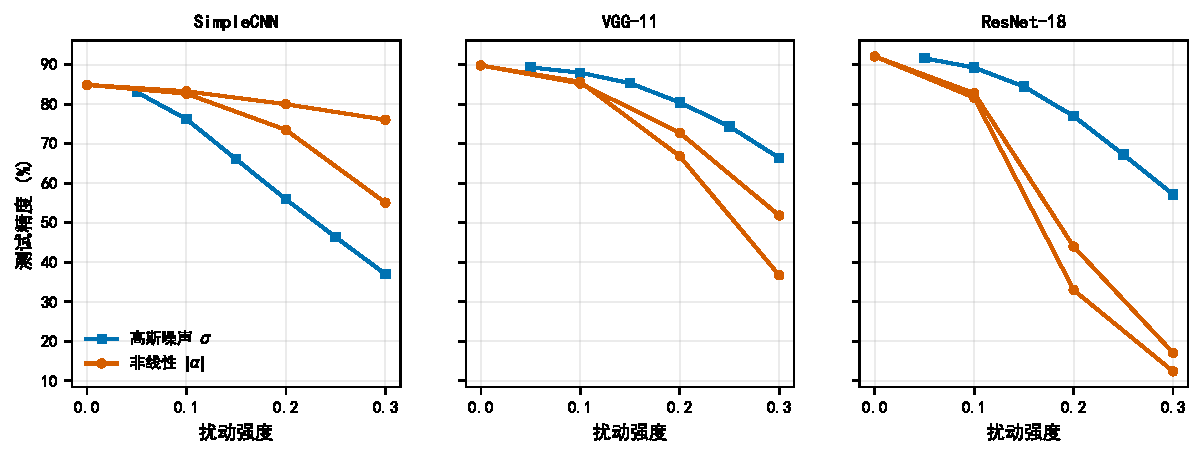
\includegraphics[width=0.98\textwidth]{C04_task_ext2_gauss_vs_nonlin.pdf}
\caption{非线性失真与加性高斯噪声的对照（CIFAR-10）。
横轴为扰动强度（高斯的 $\sigma$ 与非线性的 $|\alpha|$）。
三种架构上的排序完全不同：SimpleCNN 对高斯更脆弱，ResNet-18 则对非线性更脆弱。
数据：\texttt{outputs/extension2\_*/.../\{gaussian,nonlinearity\}\_sensitivity.csv}。}
\label{fig:c04}
\end{figure}

\begin{table}[t]
\centering
\caption{两种扰动在强度 0.3 下的精度对照（CIFAR-10）}
\label{tab:gauss}
\small
\begin{tabular}{lccc}
\toprule
架构 & 干净 & 高斯 $\sigma=0.3$ & 非线性 $\alpha=+0.3$ \\
\midrule
SimpleCNN & 84.90 & \textbf{37.02} & 55.08 \\
VGG-11 & 89.80 & 66.39 & \textbf{36.70} \\
ResNet-18 & 92.09 & 57.15 & \textbf{17.08} \\
\bottomrule
\end{tabular}
\end{table}

\cref{tab:gauss} 显示三者的排序完全不同，其中 ResNet-18 上两种扰动\textbf{完全反转}：
它对高斯噪声几乎免疫（57.15\%），却对非线性失真近乎崩溃（17.08\%）。
原因在于残差连接对两种扰动的作用方向相反——
对零均值的随机噪声，加法路径起平均化作用（缓冲）；对信号相关的确定性失真，
它起叠加放大作用。

\textbf{结论是负面的但重要}：非线性失真与高斯噪声的鲁棒性\textbf{不可跨域迁移}。
针对高斯噪声设计的方法不能期待在非线性失真下有效。
（后续阶段补充：这条"不可迁移"\textbf{是架构依赖的}——在 MaxPool 密集的 VGG-11 上迁移非零，
$\max|\Delta_\sigma|=5.26$；本稿的"不可迁移"结论限于本稿覆盖的架构。）

\subsection{拓展3：量化误差与非线性误差的联合作用}

真实 CiM 芯片在模拟域失真之外还有 ADC 量化。二者同时存在时相互放大还是抵消？
本文按物理路径顺序注入（先模拟域非线性，再数字域量化），
用"乘性独立预测"作为基准：
\begin{equation}
\text{独立预测}(\text{bit}) = \frac{a_{\text{nl}}(\alpha{=}0.3)\times a_{\text{quant}}(\text{bit})}{a_{\text{clean}}},
\qquad
\Delta = a_{\text{joint}}(\alpha{=}0.3,\text{bit}) - \text{独立预测}(\text{bit}).
\end{equation}
$\Delta<-1$ 记为超加性（比独立更差），$\Delta>+1$ 记为次加性（比独立更好）。

\begin{figure}[t]
\centering
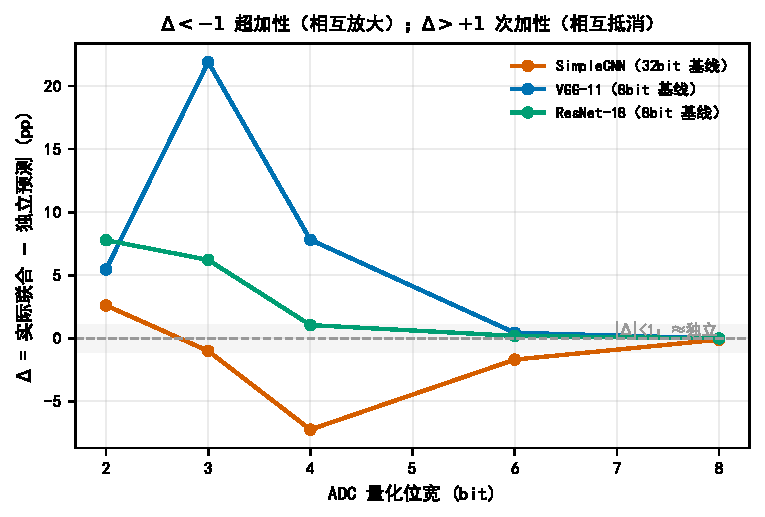
\includegraphics[width=0.72\textwidth]{C05_task_ext3_joint.pdf}
\caption{量化与非线性联合作用的加性裁决（CIFAR-10，$\alpha=+0.3$）。
灰色带为 $|\Delta|<1$ 的"近似独立"区间。
SimpleCNN 在 4bit 处超加性恶化（$\Delta=-7.23$），
VGG-11 在 3--4bit 处次加性（Dithering），ResNet-18 全程近似独立（地板效应）。
数据：\texttt{outputs/extension3\_*/joint\_error\_summary.csv}。}
\label{fig:c05}
\end{figure}

\cref{fig:c05} 给出一个\textbf{三分格局}：

\begin{itemize}[leftmargin=2em,itemsep=2pt]
  \item \textbf{SimpleCNN —— 超加性恶化}。4 bit 处 $\Delta=-7.23$：两种误差相互放大，必须同时防御。
  \item \textbf{VGG-11 —— 次加性（Dithering）}。4 bit 处 $\Delta=+7.82$：量化噪声反而\textbf{改善了}
        失真下的精度；3 bit 处幅度更大（$+21.90$）但绝对精度已经腰斩。
  \item \textbf{ResNet-18 —— 地板效应}。各 bit 下精度都在 17\% 附近，
        独立预测也在同一量级，差异无意义。
\end{itemize}

高位量化在两端都近似无损（8 bit 处 $\Delta$ 分别为 $-0.10$ 与 $0.00$），
说明"量化误差与非线性的独立叠加"是高位下的正确图景，
非线性才是主要误差源。

\section{第二阶段优化一：外推边界}
\label{sec:ext4}

\subsection{问题}

第一阶段的所有鲁棒性结论都建立在 $\alpha\in[-0.3,0.3]$ 之内，
而这正是训练时的采样分布。如果部署环境的实际失真超出这个范围，
防御手段是否仍然有效？本节把扫描范围扩大一倍到 $\pm0.6$，
把评估域分成\textbf{训练区间}（$|\alpha|\le0.3$）与\textbf{外推区}（$|\alpha|>0.3$）。

\subsection{非线性感知训练的鲁棒性是分布内属性}

\begin{figure}[t]
\centering
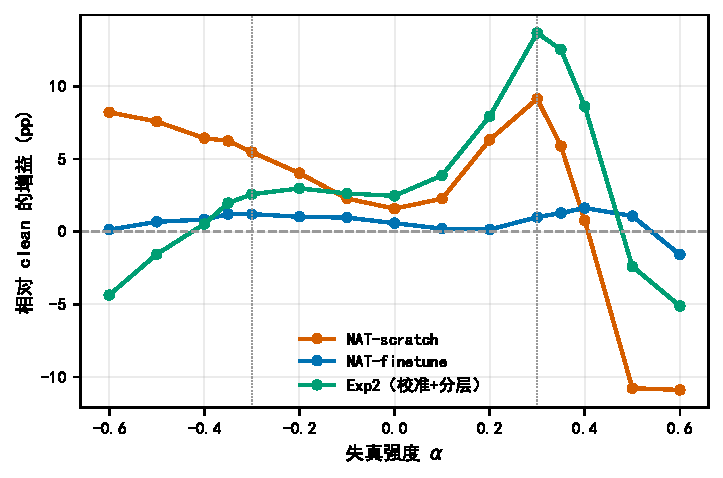
\includegraphics[width=0.72\textwidth]{C08_ext4_extrapolation.pdf}
\caption{非线性感知训练的收益严格限定在训练分布之内（CIFAR-10 / SimpleCNN）。
纵轴为相对同架构干净模型的增益；竖直虚线标出训练区间 $\pm0.3$。
Scratch 策略在正侧外推区迅速归零（$\alpha=+0.4$ 时 $+0.77$）
并反转为劣势（$\alpha=+0.5$ 时 $-10.77$），而负侧保持正值。
数据：\texttt{outputs/extension4\_alpha\_wide/alpha\_wide\_scan\_summary.csv}。}
\label{fig:c08}
\end{figure}

\cref{fig:c08} 给出一个清晰的交叉现象。
从头训练（Scratch）策略的增益随外推距离\textbf{单调衰减}：
$+9.15$（$\alpha=+0.3$）$\to +0.77$（$+0.4$，归零）$\to -10.77$（$+0.5$，反转为劣势）。
也就是说，在失真环境中过度适应的模型，
在更极端的失真下其表征反而比"从未见过失真"的干净模型更脆弱。

微调策略的外推衰减最缓——它是三种权重中唯一在 $\alpha=+0.4$ 与 $+0.5$ 处仍不恶化的
（$+1.63$ / $+1.08$）；到最外端 $\alpha=+0.6$ 才转为 $-1.58$，但仍远优于 Scratch 的 $-10.89$。
这与第一阶段"ResNet-18 极限失真下微调反超从头训练"的观察在机理上一致：
低学习率保留下来的干净特征编码，恰是分布外场景的稳定基础。

\subsection{负向外推保持，不对称性再证}

与正侧形成鲜明对照：Scratch 在负侧的增益随外推距离\textbf{不降反升}
（从 $+5.48$ 升至 $\alpha=-0.6$ 处的 $+8.22$），VGG-11 在负侧全区间保持 $+5\sim14$ 个百分点。
这与第一阶段的"正向破坏力更强"同向：
正方向是本质上的难防御方向。

\subsection{架构容差窗口随深度收窄}

干净模型能保持可用精度（$\ge70\%$）的 $\alpha$ 窗口为：
SimpleCNN 约 $[-0.35,+0.25] >$ VGG-11 约 $[-0.25,+0.2] >$ ResNet-18 约 $[-0.15,+0.15]$。
深层网络不仅极限失真下崩溃，其\textbf{可容忍失真带宽本身就更窄}——
这直接论证了优化三（深层迁移）的必要性。

\section{第二阶段优化二：Dithering 效应的定量机理}
\label{sec:ext5}

\subsection{一个需要解释的反常现象}

第一阶段发现：VGG-11 在 $\alpha=+0.3$ 失真下，
4 bit 量化的精度（43.27\%）反而\textbf{高于} 8 bit（36.74\%），增益 $+6.53$ 个百分点，
且为 VGG-11 独有。当时把它解释为"随机共振/抖动去相关"，
并据此提出"在 ADC 前注入随机噪声"的工程建议——\textbf{该解释未经实验检验}。

\begin{figure}[t]
\centering
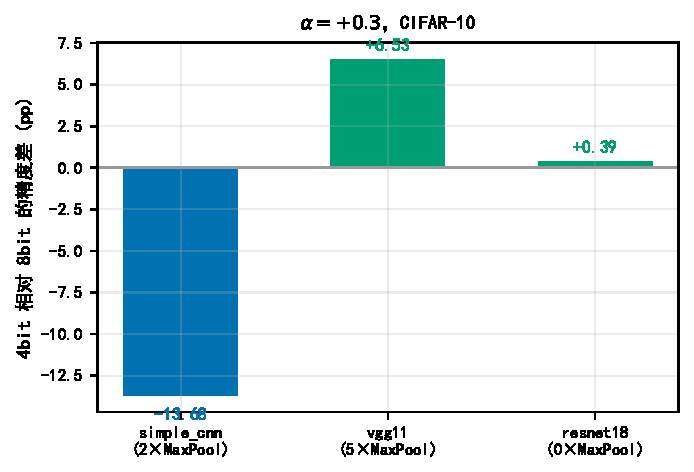
\includegraphics[width=0.62\textwidth]{C06_dithering_arch.pdf}
\caption{Dithering 增益的架构依赖（CIFAR-10，$\alpha=+0.3$）。
横轴上标注每个架构的 MaxPool 数量。增益与 MaxPool 密度同向但要足够密——
2 个 MaxPool 的 SimpleCNN 是负增益，0 个的 ResNet-18 无效应。
数据：\texttt{outputs/extension5\_dithering\_vgg11/arch\_dithering\_summary.csv}。}
\label{fig:c06}
\end{figure}

\subsection{三假设竞争判决}

本节设计三个互斥的假设与相应判决信号：

\begin{center}
\small
\begin{tabular}{clp{7.6cm}}
\toprule
假设 & 机理表述 & 判决信号 \\
\midrule
H1 & 随机去相关：随机扰动打破失真的确定性错误映射 & 等剂量随机噪声若能复现增益则支持 \\[2pt]
H2 & 分布重塑：粗量化对失真压平的分布做非线性再分配 & 激活峰度随位宽下调而系统性恢复，且与精度关联 \\[2pt]
H3 & MaxPool 交互：局部最大值筛选与量化误差交互 & 增益随 MaxPool 密度排序 \\
\bottomrule
\end{tabular}
\end{center}

实验用\textbf{剂量匹配的三组对照}（量化 / 等剂量纯噪声 / 8bit$+$最优剂量噪声）、
样本级翻转统计（10\,000 样本逐个比对）与分类器输入分布统计，给出定量判决。

\subsection{判决结果}

\begin{table}[t]
\centering
\caption{剂量匹配三对照（VGG-11，$\alpha=+0.3$）}
\label{tab:dose}
\small
\begin{tabular}{lccc}
\toprule
条件 & 剂量 & 精度 & 相对 8bit 基线 \\
\midrule
8bit 基线 & 0.014 & 36.74 & --- \\
\textbf{4bit} & \textbf{0.245} & \textbf{43.27} & $\mathbf{+6.53}$ \\
等剂量高斯噪声 & 0.247 & 34.29 & $-2.45$ \\
等剂量均匀噪声 & 0.247 & 34.87 & $-1.87$ \\
8bit $+$ 最优剂量高斯 & 0.041 & 36.71 & $-0.03$ \\
\bottomrule
\end{tabular}
\end{table}

\textbf{H1（随机去相关）$\to$ 否决。}
\cref{tab:dose} 显示：用与 4 bit 等效剂量的纯噪声替代量化，精度\textbf{不升反降}；
在 8 bit 基线上叠加最优剂量的随机噪声，增益只有 $-0.03$ 个百分点。
样本级翻转统计给出了三个量级的反差：4 bit 的"救回:杀死"为 4.15:1（净 $+653$ 样本），
而噪声条件约为 1:1（净 $+7$ 与 $-19$）。
\textbf{随机性不是增益的来源。}

\textbf{H2（分布重塑）$\to$ 确认，核心机理。}
分类器输入分布的峰度在失真下被从 1.486 压平到 0.110（标准差同时从 0.682 降到 0.461），
可分性被破坏，精度跌到 36.74\%；
4 bit 的 16 电平粗离散化对该压平分布做非线性再分配，把峰度恢复到 \textbf{0.214}，
部分重建可分性（$+6.53$）。
存在一个甜点带：3 bit 的峰度更高（0.384）但精度略降（重塑过头叠加信息损失），
2 bit 信息量不足、峰度与精度双双坍缩。

\textbf{H3（MaxPool 交互）$\to$ 支持，必要条件。}
无 MaxPool 的 ResNet-18 完全免疫（$+0.39$），
说明 MaxPool 是效应触发的必要条件；
但只有 2 个 MaxPool 的 SimpleCNN 是\textbf{负增益}（$-13.68$），
说明它并非充分条件——\textbf{密度与位置决定量化误差是被修正还是被放大}。

\subsection{对第一阶段解释的修正}

\textbf{本节的判决否决了第一阶段的"随机共振/抖动去相关"解释，以及据此提出的
"在 ADC 前注入随机噪声"的工程建议}（等剂量注噪的增益约为零）。
正确的工程表述是：\textbf{在 MaxPool 密集的架构（VGG 类）上，
直接采用 4 bit ADC 本身即可获得失真补偿；注噪方案无效。}

同时还得到一个配方设计的警示：3 bit 的次加性幅度比 4 bit 更大（$+21.90$ 对 $+7.82$），
但绝对精度已经腰斩（42.97\% 对 43.27\%，约为干净模型 89.80\% 的一半）。
\textbf{"增益幅度"不能单独作为配方优劣的判据}，必须与绝对精度联合裁决。

\section{第二阶段优化三：增强方案向深层网络的迁移}
\label{sec:ext6}

\subsection{问题与迁移设计}

第一阶段的 Exp2 方案（残差校准模块 $+$ 分层加权采样）只在 SimpleCNN 上验证过。
本节把它完整迁移至 VGG-11 与 ResNet-18，同配方从头训练，
并顺带复验优化一发现的 Exp2 外推短板是否为该方案的固有缺陷。

校准模块的注入位置按架构适配：VGG-11 注入在每个 MaxPool 之后（5 处，
因为 MaxPool 是空间下采样与误差累积节点）；ResNet-18 注入在每个基本块的残差路径上（8 处）。
分层 $\alpha$ 的数值范围与原方案逐项一致，只按各架构深度重新映射层名。

\subsection{迁移结果}

\begin{figure}[t]
\centering
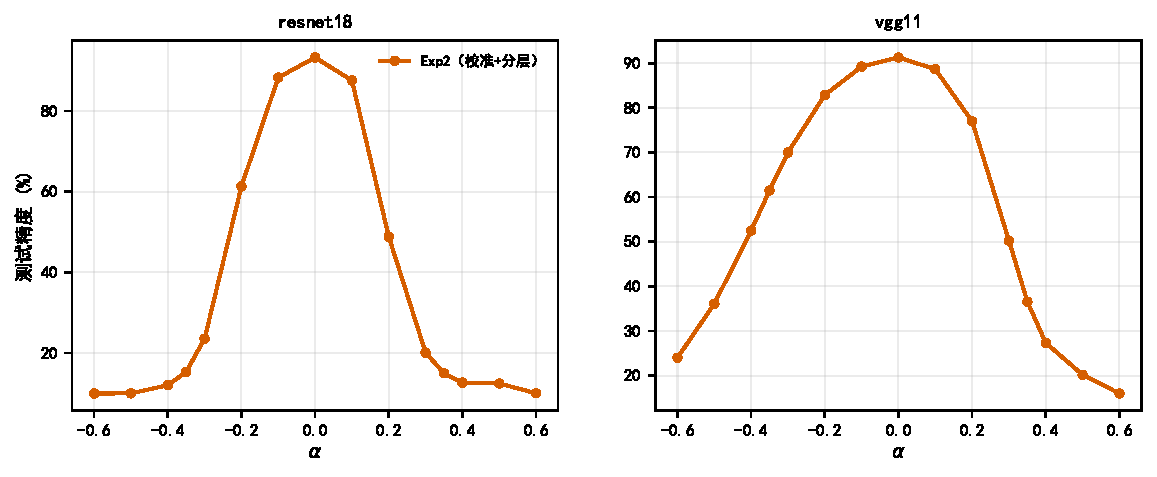
\includegraphics[width=0.90\textwidth]{C07_ext6_deep_transfer.pdf}
\caption{Exp2 增强方案向深层主干迁移（CIFAR-10）。
灰色虚线为同架构干净模型，橙色为 Exp2 方案（残差校准 $+$ 分层加权）。
在 VGG-11 上，Exp2 在全部 15 个扫描点上都优于三条基线；
在 ResNet-18 上全程无败，但正侧强失真区的绝对精度仍然很低。
数据：\texttt{outputs/extension6\_deep\_robust/alpha\_wide\_scan\_deep\_robust.csv}。}
\label{fig:c07}
\end{figure}

\begin{table}[t]
\centering
\caption{Exp2 方案迁移后的关键精度（CIFAR-10，\%）}
\label{tab:transfer}
\small
\begin{tabular}{llccc}
\toprule
架构 & 权重 & $\alpha=0$ & $\alpha=+0.3$ & 相对 clean \\
\midrule
VGG-11 & clean & 89.80 & 36.70 & --- \\
VGG-11 & NAT-scratch & 90.18 & 44.74 & $+8.04$ \\
VGG-11 & \textbf{Exp2} & \textbf{91.27} & \textbf{50.25} & $\mathbf{+13.55}$ \\
\midrule
ResNet-18 & clean & 92.09 & 17.08 & --- \\
ResNet-18 & NAT-scratch & 92.27 & 15.64 & $-1.44$ \\
ResNet-18 & \textbf{Exp2} & \textbf{93.27} & \textbf{20.12} & $\mathbf{+3.04}$ \\
\bottomrule
\end{tabular}
\end{table}

\cref{tab:transfer} 与 \cref{fig:c07} 给出四项发现：

\textbf{(1) 增益跨架构传递。}
$\alpha=+0.3$ 相对干净模型的增益为 $+13.68$（SimpleCNN）$\to +13.55$（VGG-11）$\to +3.04$（ResNet-18）。
VGG-11 与 SimpleCNN 几乎无损传递，说明方案的有效性不依赖浅层架构。

\textbf{(2) 多点校准修复了外推短板。}
SimpleCNN 上的 Exp2 采用单一注入点（全局池化之后），
在负侧外推区输给 NAT-Scratch 最多 12.58 个百分点；
深层版本采用 5/8 个空间注入点后，在\textbf{15 个扫描点上全部压制 NAT-Scratch}。
结论是：单一注入点的校准容量不足是外推短板的成因，多点空间校准可以修复它。

\textbf{(3) 增益随深度衰减，机制是复合最坏情形。}
逐层独立采样下，训练时所有层同时取到极端 $\alpha$ 的概率趋近于零；
而评估时全局 $\alpha=+0.3$ 意味着 ResNet-18 的全部 17 个卷积层\textbf{同时}处于边界失真——
这是训练分布之外的尾部事件，层数越多越极端。

\textbf{(4) 干净精度零牺牲。}
两个架构 Exp2 的 $\alpha=0$ 精度（91.27 / 93.27）都是四组权重中最高的，
校准模块兼具正则化作用。

此外，ResNet-18 上 Exp2 的 20.12\% 反超了第一阶段的"改用微调"策略（19.89\%），
说明\textbf{架构级校准可以恢复从头训练策略在残差网络上的竞争力}。

\section{讨论与结论}

\subsection{贯穿两阶段的三条主线}

\textbf{主线一：正负不对称性。}
三个阶段、四类实验都指向同一结论——正向失真是本质上的难防御方向：
破坏力不对称（任务1 的 3.4 倍）、外推不对称（优化一：负侧保持而正侧反转）、
防御不对称（优化三：三架构上 Exp2 的负侧精度都显著高于正侧）。
工程含义是补偿资源应向正方向倾斜；但也解释了为何非对称采样（方案 C）边际收益小——
瓶颈不在采样比例，而在表征能力。

\textbf{主线二：深度的复合放大。}
注入点数 5$\to$9$\to$18 对应脆弱性递增、非线性感知训练的临界阈值约 10 个注入点、
容差窗口随深度收窄、增益随深度衰减——
统一解释是\textbf{复合最坏情形概率随深度指数放大}，
无论评估端（全层同失真）还是训练端（独立采样的覆盖不足）。
可操作的工程判据：注入点超过约 10 个的架构，必须配合多点校准才可期待有效防御。

\textbf{主线三：校准注入密度应随误差累积节点数扩展。}
单点校准（SimpleCNN 的 1 处）负侧外推输 12.58 个百分点，
多点校准（深层 5/8 处）15 点全胜。
校准密度必须与误差累积节点数同步扩展，单点校准只保护分类边界，不保护特征通路。

\subsection{结论}

本文在 CIFAR-10 上系统考察了模拟域非线性失真对神经网络的影响与应对，主要结论：

\begin{enumerate}[leftmargin=2em,itemsep=2pt]
  \item 正向失真的破坏力在浅层主干上强于负向（SimpleCNN 上为 3.4 倍），
        \textbf{但方向性随深度衰减、在最深的主干上消失}（ResNet-18 上为 0.94）；
        误差从浅层向深层超加性累积，残差连接是误差放大器，ResNet-18 在 $\alpha=+0.3$ 下损失 75 个百分点。
  \item 非线性感知训练在纯前馈网络上有效（$+8\sim9$ 个百分点），
        在残差网络极限失真下失效（$-1.44$）；效果与注入点数量负相关。
  \item 叠加残差校准模块与分层加权采样后，SimpleCNN 的 $\alpha=+0.3$ 达 \textbf{68.76\%}，
        且干净精度不降反升；分层加权是贡献最大的单项（$+5.13$）。
  \item 非线性失真与高斯噪声的鲁棒性\textbf{不可跨域迁移}（\textbf{架构依赖}：
        在 MaxPool 密集的 VGG-11 上迁移非零，$\max|\Delta_\sigma|=5.26$），
        两者在 ResNet-18 上的排序完全反转。
  \item 量化与非线性的联合作用呈三分格局：超加性 / 次加性（Dithering）/ 地板效应。
  \item \textbf{非线性感知训练的鲁棒性是训练分布内的属性}：
        正向外推在 $\alpha\approx0.4$ 处归零并转为劣势，负向外推保持。
  \item \textbf{Dithering 的机理是离散化分布重塑配合 MaxPool 架构载体，
        与随机性无关}——第一阶段给出的"随机共振"解释与注噪建议已被否决。
  \item Exp2 方案可完整迁移至深层网络（VGG-11 全点全胜），
        多点校准修复了单点版本的外推短板，且干净精度零牺牲。
\end{enumerate}

\subsection{局限与后续方向}

\textbf{局限}：三项拓展的数据集多样性（评审建议 R4）\textbf{不在本稿范围内}（见文首范围声明）；
校准模块的机理证据是相关性证据（峰度-精度关联与架构对照），
未做因果干预实验（如逐层替换 MaxPool 为平均池化）；
残差网络正侧强失真区的绝对精度仍然很低（20.12\%），
根因是逐层独立采样无法覆盖复合最坏情形。

\textbf{后续方向}：① 层间相关或对抗式的 $\alpha$ 采样，
以覆盖"所有层同时处于边界"这一尾部事件；
② 把数据集多样性补上，检验上述规律在细粒度任务上是否保持；
③ 探索不依赖训练手段、也不依赖网络重训的修复路径
（本文的全部方法都需要改动网络或重新训练，
而在真实的存算一体部署中，阵列里的权重是不可重训的）。

\begin{thebibliography}{99}
\bibitem{cim_survey} Yu S, Chen P Y. Emerging memory technologies: recent trends and prospects[J]. IEEE Solid-State Circuits Magazine, 2016, 8(2): 43--56.
\bibitem{puma} Ankit A, El Hajj I, Chalamalasetti S R, et al. PUMA: a programmable ultra-efficient memristor-based accelerator for machine learning inference[C]//ASPLOS. Providence: ACM, 2019: 715--731.
\bibitem{vgg} Simonyan K, Zisserman A. Very deep convolutional networks for large-scale image recognition[C]//ICLR. San Diego: ICLR, 2015: 1--14.
\bibitem{resnet} He K, Zhang X, Ren S, et al. Deep residual learning for image recognition[C]//CVPR. Las Vegas: IEEE, 2016: 770--778.
\bibitem{cifar} Krizhevsky A. Learning multiple layers of features from tiny images[R]. Toronto: University of Toronto, 2009.
\bibitem{neat} Bhattacharjee A, Bhatnagar L, Kim Y, et al. NEAT: nonlinearity aware training for accurate, energy-efficient, and robust implementation of neural networks on 1T-1R crossbars[J]. IEEE TCAD, 2022, 41(8): 2625--2637.
\bibitem{quant} Jacob B, Kligys S, Chen B, et al. Quantization and training of neural networks for efficient integer-arithmetic-only inference[C]//CVPR. Salt Lake City: IEEE, 2018: 2704--2713.
\bibitem{dither} Wannamaker R A, Lipshitz S P, Vanderkooy J, et al. A theory of nonsubtractive dither[J]. IEEE Transactions on Signal Processing, 2000, 48(2): 499--516.
\end{thebibliography}

\end{document}
